\documentclass[crop=false]{standalone}
\begin{document}
	\section{System Overview}
	
	系統架構如圖一所示,由RGBD攝影機拍攝具有深度影像資訊後,將RGB影像與深度影像輸入進YOLO物件偵測模型。交由深度學習模型負責執行物件偵測,再由模型偵測到的物件位置轉換座標系後給DWA動態調整路徑。此外,加入最短路徑演算法,提升 DWA在評選路徑時的速度。此最短路徑能使得無人機以最少時間情況下抵達指定的地點,並且能夠避開障礙物。
	
	\begin{figure*}[thbp!]
		\centering
		\fbox{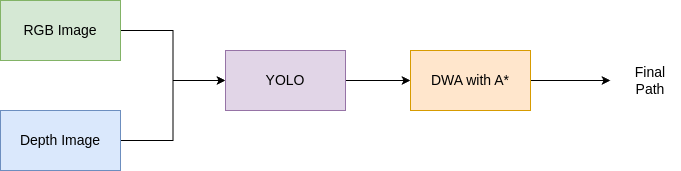
\includegraphics[width=\textwidth]{furtherwork_workflow}}
		\caption{The system architecture}
		\label{fig:system}
	\end{figure*}
\end{document}